\documentclass[../Cours.tex]{subfiles}

\usepackage{xstring}
\usepackage{xfp}

\begin{document}
\clearpage
\thispagestyle{empty}

\setcounter{DS}{1}

\color{black}
\nomPrenom
\titreDS

\begin{questions}
    \EXERCICETITRE{4}{DISTANCE D'ARRÊT}
    \bionic[0.4]{Lorsque le conducteur d'un véhicule perçoit un obstacle et veut freiner, il va d'abord avoir un temps de réaction d'une seconde ; cette distance est appelée distance de réaction. Puis, il va appuyer sur la pédale de frein, et la voiture va freiner sur une certaine distance appelée distance de freinage.\\
    La distance d'arrêt est la somme de la distance de réaction et de la distance de freinage.}\\ 

    \question Si une voiture roule à \qty{20}{\metre\per\second}, quelle est sa distance de réaction ?

    \caseReponse{2.5}

    \begin{center}
    \begin{tikzpicture}
        \node[anchor=west] at (-2,1.5) {Pour calculer la distance de freinage, on utilise la formule :};
        \node at (2.5,-0.5) {$D_f = \dfrac{v^2}{2 \times g \times a}$};
        \node[anchor=west] at (6.5,0) {$v$ est la vitesse (en \unit{\metre\per\second})};
        \node[anchor=west] at (6.5,-0.6) {$g = 10$};
        \node[anchor=west] at (6.5,-1.2) {$a = 0,8$ sur route sèche, $a = 0,6$ sur route mouillée};
        \draw[dotted] (-2,1.8) rectangle (16,-2);
    \end{tikzpicture}
    \end{center}
    \question Si une voiture roule à \qty{20}{\metre\per\second} sur route mouillée, quelle est sa distance de freinage ?
    \caseReponse{2}
    \question En déduire sa distance d'arrêt.
    \caseReponse{2}

    \clearpage

    \EXERCICETITRE{4}{Dame blanche}
    \bionic[0.4]{Une dame blanche est un dessert composée de deux boules de glace à la vanille et d'une boule de glace au chocolat.}\\

    \question Sachant que toutes les boules de glaces ont pour rayon $\qty{5}{cm}$, quel est le volume d'une boule de glace ? (Rappel : $V_{\mbox{boule}} = \frac{4}{3} \pi \times \mbox{rayon}^3$)
    \caseReponse{2}
    \question Pour faire une dame blanche, quelle volume de glace faudra-t-il utiliser au total ? On donnera le résultat en \unit{\centi\metre\cubed} et en \unit{litre}.
    \caseReponse{2}

    \EXERCICETITRE{6}{Comparaison des émissions de $CO_2$}
    \bionic[0.4]{En moyenne sur l'année 2021, pour produire un kilowattheure d'électricité, la France émet soixante-dix-huit grammes de dioxyde de carbonne tandis que l'Allemagne émet quatre cent soixante-trois grammes de dioxyde de carbonne.}\\

    \question Expliquer pourquoi l'Allemagne a une électricité 6 fois plus polluante en 2021.
    \caseReponse{2}
    \question En France, en 2021, à combien de kilowattheures correspond une 1 tonne de $CO_2$ (sachant qu'une tonne vaut $\qty{1000000}{g}$) ?
    \caseReponse{2}
    \question En Allemagne, en 2021, quelle quantité de $CO_2$ sera émise si ce pays produit \num{2500} kilowattheures ?
    \caseReponse{2}

    \clearpage
    \EXERCICETITRE{4}{Composition de l'air}
    \bionic[0.3]{Sur Terre, l'air est principalement composé de deux gaz : le diazote et le dioxygène, qui sont répartis selon le ration 4:1.}

    \question Une salle de classe a la forme d'un pavé droit. Si elle a une longueur $L=\qty{7}{m}$, une largeur $l=\qty{5}{m}$ et une hauteur de $h=\qty{3}{m}$, montrer que son volume vaut $\qty{105}{m\cubed}$.
    \caseReponse{2}
    \question Si la salle est complètement vide et n'est constituée que d'air, quelle est le volume de dioxygène et de diazote présent dans la pièce ? On donnera les réponses en \unit{\metre\cubed}.
    \caseReponse{2}

    \EXERCICETITRE{4}{Symétries}

    \question Construire un carré $ABCD$ de côté \qty{2}{\centi\metre}
    \question Construire la droite $(d)$ parallèle à la diagonale $[AC]$ passant par $D$.
    \question Construire le symétrique $A'B'C'D'$ de $ABCD$ par rapport à la droite $(d)$

    \caseReponse{6}

    \EXERCICETITRE{2}{Une grande multiplication}

    \question On multiplie tous les nombres impairs de 1 à 2017. Quel est le chiffre des unités du résultat ?
    \caseReponse{2}

    
    
\end{questions}
\end{document}